\section{Diseño de los programas}
\subsection{Diagrama de flujo del sismógrafo}
El sismógrafo se puede implementar en la placa de desarrollo STM32F429 Discovery siguiendo el diagrama de flujo que se ilustra en la figura \ref{fsm}. Por un lado, se debe inicializar todos los periféricos que se utilizarán para este laboratorio, esto es, configurar los registros de ADC, GPIO, LCD, SPI, SDRAM y USART. Luego, se leen los datos del giroscopio y la tensión de la batería para ser mostrado inmediatamente en la pantalla LCD. Estos datos serán transmitido por USART si está habilitado el pin de habilitación USART. En caso que se transmita por USART, un LED verde parpadeará. También, un LED rojo parpadeará si la tensión de la batería leida es menor a \SI{8}{\volt}. Todo el código del sismógrafo fue basado en ejemplos proporcionados por la librería \tt{libopencm3}, así que créditos a Karl
Palsson, Piotr Esden-Tempski y Chuck McManis por proporcionar dichos ejemplos \cite{libopencm3}.
\begin{figure}[H]
    \centering
    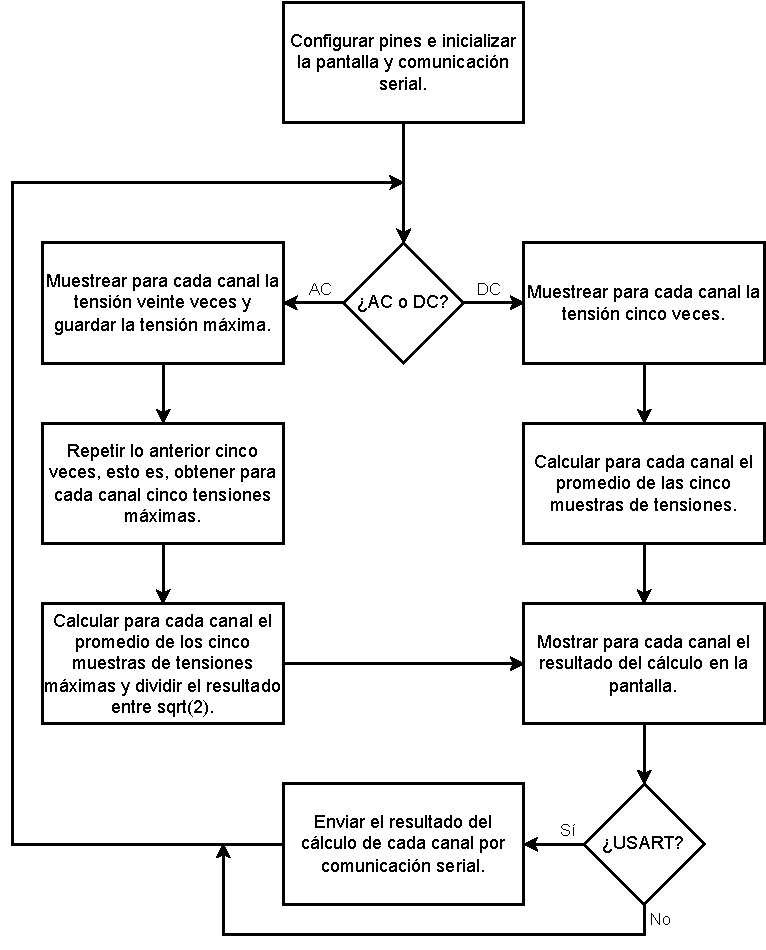
\includegraphics[width=14cm]{Imagenes/fsm.pdf}
    \caption{Diagrama de flujo del programa en el STM32F429 Discovery.}
    \label{fsm}
\end{figure}

Ahora, en la figura \ref{fsm-py} se ilustra el diagrama de flujo del programa utilizado para recibir las lecturas por comunicación serial y reenviarlos a \tt{iot.eie.ucr.ac.cr} en formato JSON. La implementación para configurar y abrir el puerto serial así como mqtt en Python se puede consultar en \cite{serial, mqtt}.
\subsection{Diagrama de flujo del programa en Python}
\begin{figure}[H]
    \centering
    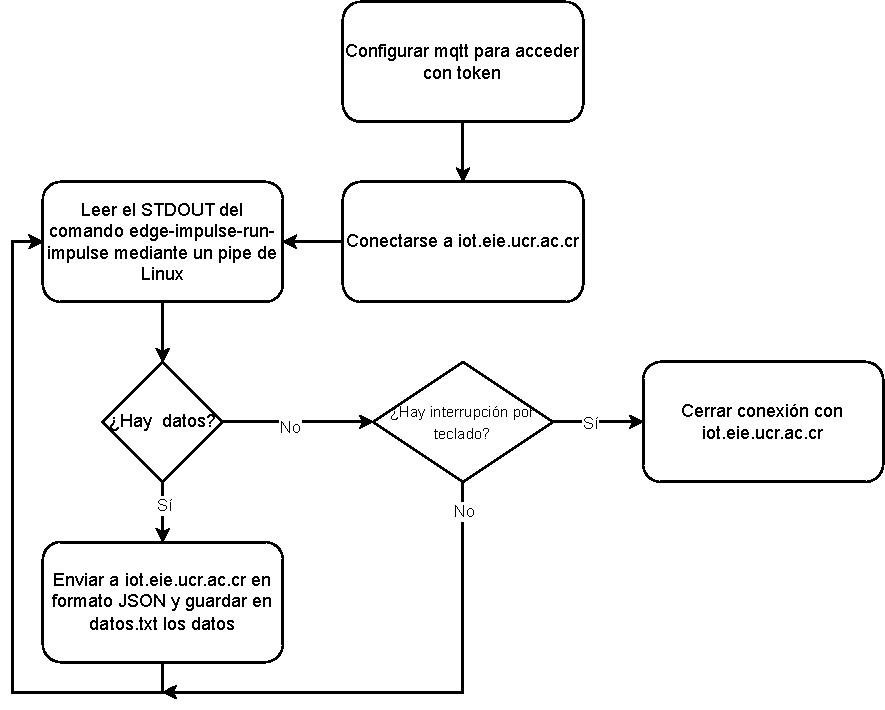
\includegraphics[width=12cm]{Imagenes/py.pdf}
    \caption{Diagrama de flujo del programa en Python que captura las lecturas de la placa desarrollo y los envía a \tt{iot.eie.ucr.ac.cr}.}
    \label{fsm-py}
\end{figure}